\documentclass[notheorems]{beamer}
\setbeamertemplate{caption}[numbered]
%\usepackage{subfig}
\usepackage[ruled,vlined,spanish]{algorithm2e}
\usepackage{amsthm}
\usepackage{amssymb}
\usepackage{array}
\usepackage[spanish]{babel}
\usepackage{blkarray}
\usepackage{bm}
\usepackage{booktabs}
\usepackage{caption}
\usepackage{float}
\usepackage{graphicx}
\usepackage[utf8]{inputenc}
\usepackage{mathtools}
\usepackage{setspace}
\usepackage{subcaption}
\newcommand{\figura}[3]{\begin{figure}[H] \centering \includegraphics[#3]{#1} \caption{#2} \label{#1}  \end{figure}}
\newcommand{\tablasimple}[2]{\begin{table}[H] \centering \input{#1} \caption{#2} \label{#1} \end{table}}
\newcommand{\tablalarga}[2]{ \begin{center} \input{#1} \begin{table}[H] \caption{#2} \label{#1} \end{table} \end{center}}
\usetheme{CambridgeUS}
\usecolortheme{seahorse}
\institute[]{Statistical Machine Learning \\ Profa. Guillermina Eslava \\ Posgrado en Ciencias Matemáticas \\ Universidad Nacional Autónoma de México}
\author{César Cossio Guerrero. Aldo Sayeg Pasos Trejo}
\date{\today}
\title[Tarea-examen 5-6]{Tarea-examen 5-6: selección de modelos y regularización}
\begin{document}

\begin{frame}
    \maketitle
\end{frame}
\begin{frame}{Problema 1: Modelo normal}
        \tablasimple{base.tex}{Estadísticas del modelo base. Los errores no aparentes se calcularon mediante validación cruzada con $k=5$ y $100$ repeticiones}
\end{frame}
\begin{frame}{Problema 1: Modelos seleccionados}
    \tablasimple{modDetails.tex}{Detalles de cada modelo}
\end{frame}
\begin{frame}{Problema 1: $\lambda$ en modelos regularizados}
    \figura{regularized.pdf}{Error cuadrático medio para los modelos}{height = 0.80\textheight} 
\end{frame}
\begin{frame}{Problema 1: Variables de cada modelo}
    \figura{variables.pdf}{Variables para cada modelo}{height = 0.80\textheight}
\end{frame}
\begin{frame}{Problema 1: Errores de cada modelo}
    \begin{table}
        \begin{tabular}{p{2.5cm}|c|p{1.5cm}|p{1.5cm}|p{1.5cm}|p{1.5cm}}
            \toprule
                      model &  Dfs &    R\textasciicircum 2 &  Aparent error &  Non aparent error &  Non aparent error std \\
            \midrule
                step (AIC) &   52 & 0.9199 &         0.4245 &             0.5671 &                 0.0255 \\
                step (BIC) &   32 & 0.9107 &         0.4733 &             0.5564 &                 0.0143 \\
               Best subset &   20 & 0.8860 &         0.6043 &             0.6641 &                 0.0129 \\
                     Lasso &   25 & 0.8871 &         0.5983 &             0.6749 &                 0.0126 \\
                     Ridge &   92 & 0.8824 &         0.6234 &             0.7304 &                 0.0125 \\
               Elastic Net &   31 & 0.8881 &         0.5934 &             0.6772 &                 0.0129 \\
             Random Forest &   91 & 0.9929 &         0.0378 &             0.3039 &                 0.0123 \\
            \bottomrule
        \end{tabular}
        \caption{Errores para cada modelo}
    \end{table}
\end{frame}
\begin{frame}{Problema 1: Modelos seleccionados por step}
    \begin{table}
        \begin{tabular}{p{2cm}|p{1.5cm}|p{1.5cm}|p{1.5cm}|p{1.5cm}}
            \toprule
                  model &  Selection outside CV &  Selection outside CV std &  Selection inside CV &  Selection inside CV std \\
            \midrule
             step (AIC) &                0.5671 &                    0.0255 &               1.5123 &                   0.1992 \\
             step (BIC) &                0.5564 &                    0.0143 &               1.3623 &                   0.3950 \\
            \bottomrule
        \end{tabular}
        \caption{Errores incluyendo proceso de selección}
    \end{table}
\end{frame}
\begin{frame}{Problema 2: Modelo Ridge}
    \begin{figure}
    \centering
    \subfloat{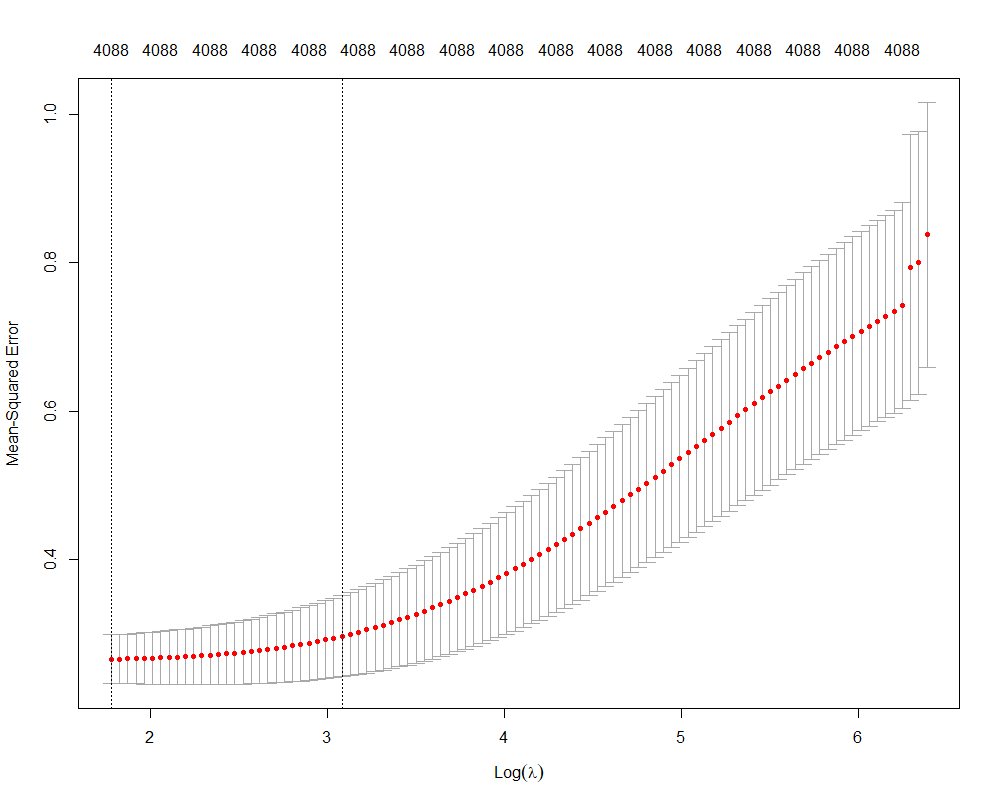
\includegraphics[width=0.48\textwidth]{MS1.png}}
    \subfloat{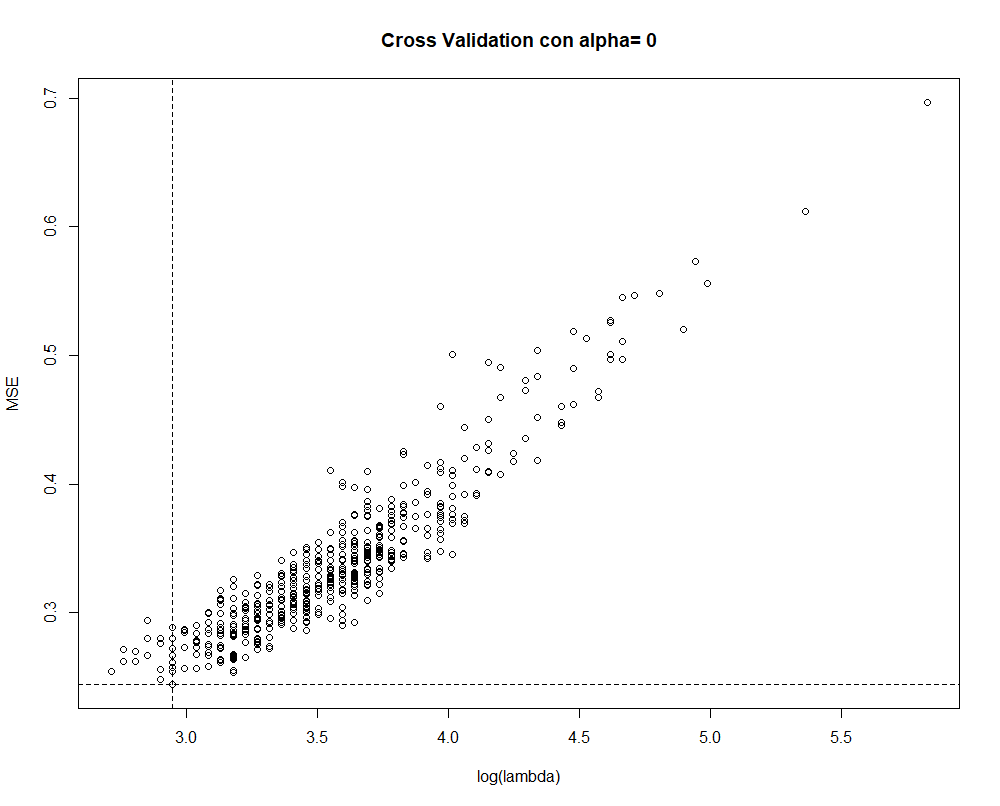
\includegraphics[width=0.48\textwidth]{MSCV1.png}} 
        \caption{}
    \end{figure}
\end{frame}
\begin{frame}{Problema 2: Modelo Elastic Net}
    \begin{figure}
    \centering
    \subfloat{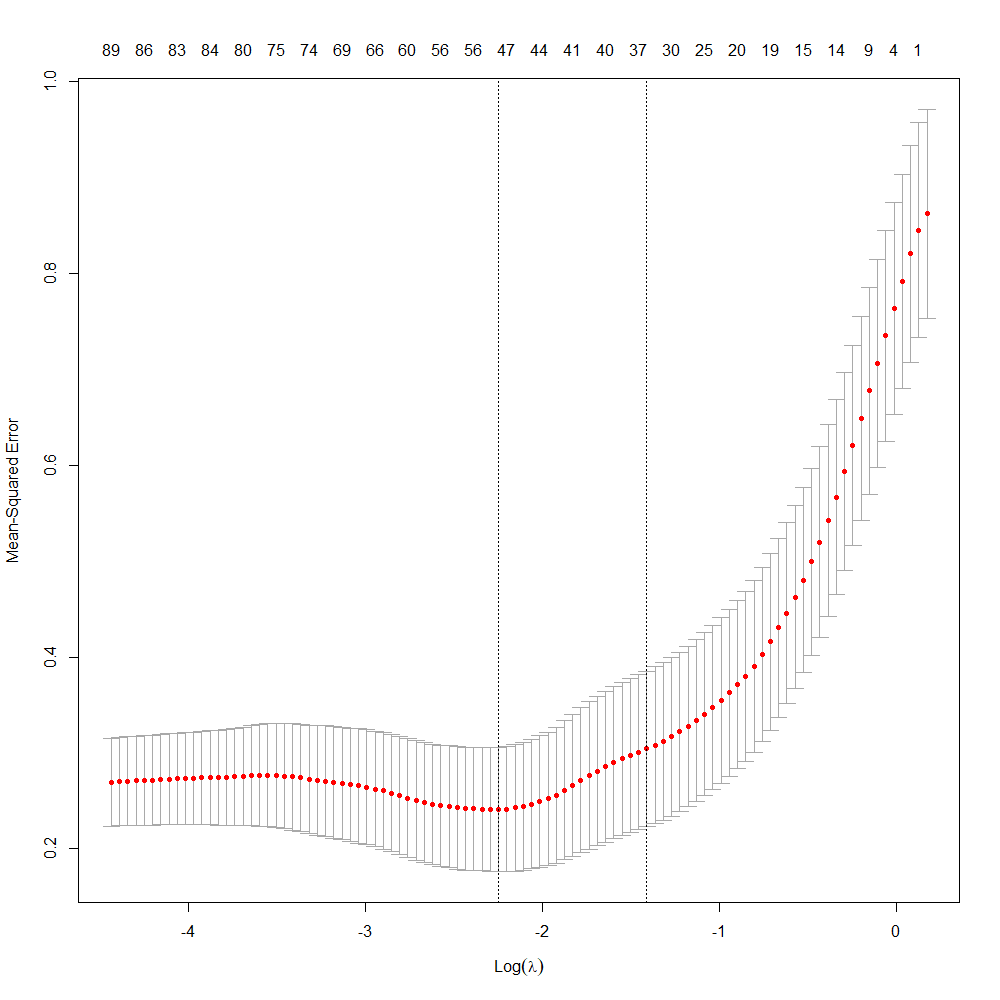
\includegraphics[width=0.48\textwidth]{MS2.png}}
    \subfloat{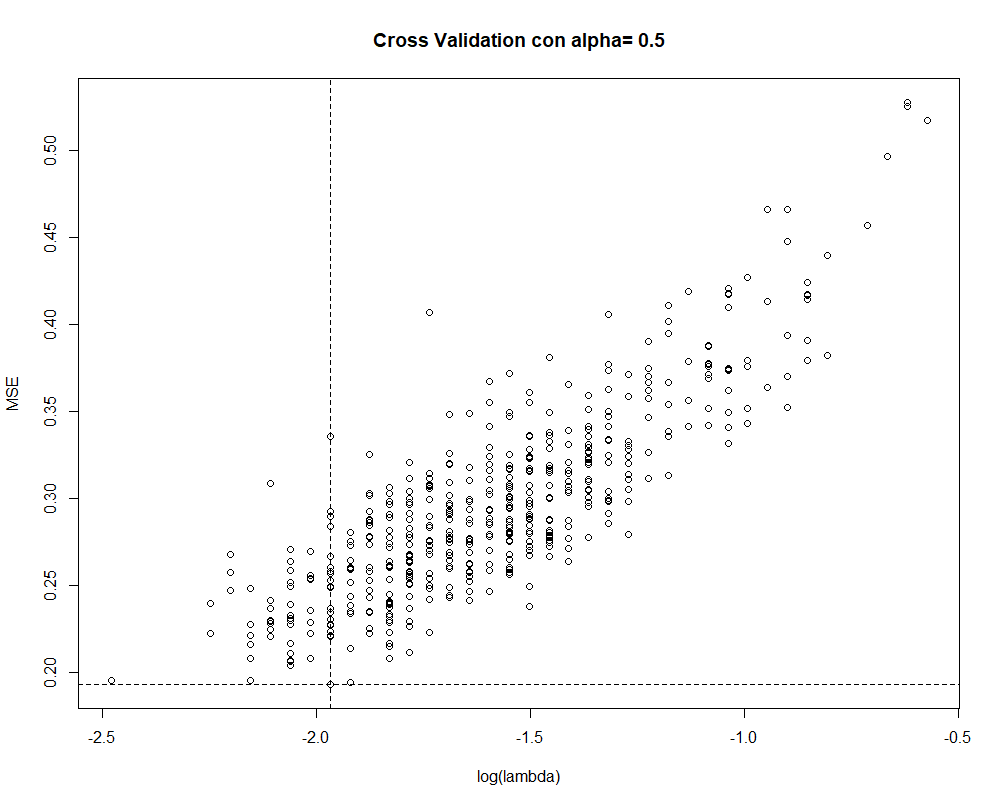
\includegraphics[width=0.48\textwidth]{MSCV2.png}} 
        \caption{}
    \end{figure}
\end{frame}
\begin{frame}{Problema 2: Modelo Elastic Net}
    \begin{figure}
    \centering
    \subfloat{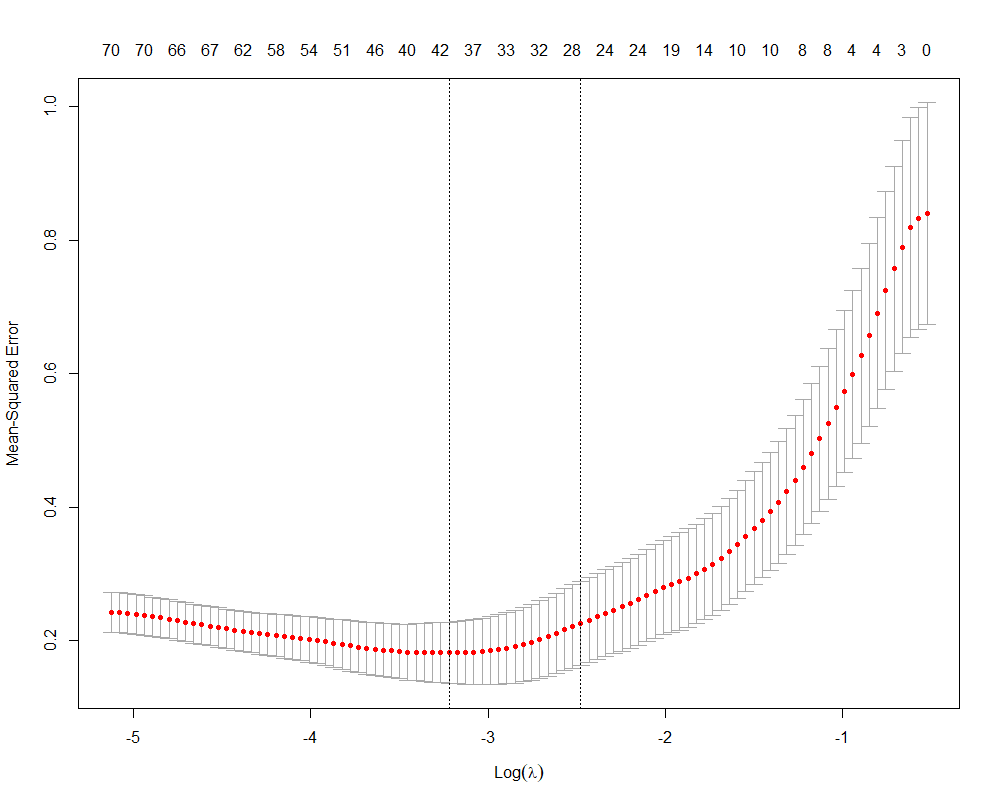
\includegraphics[width=0.48\textwidth]{MS3.png}}
    \subfloat{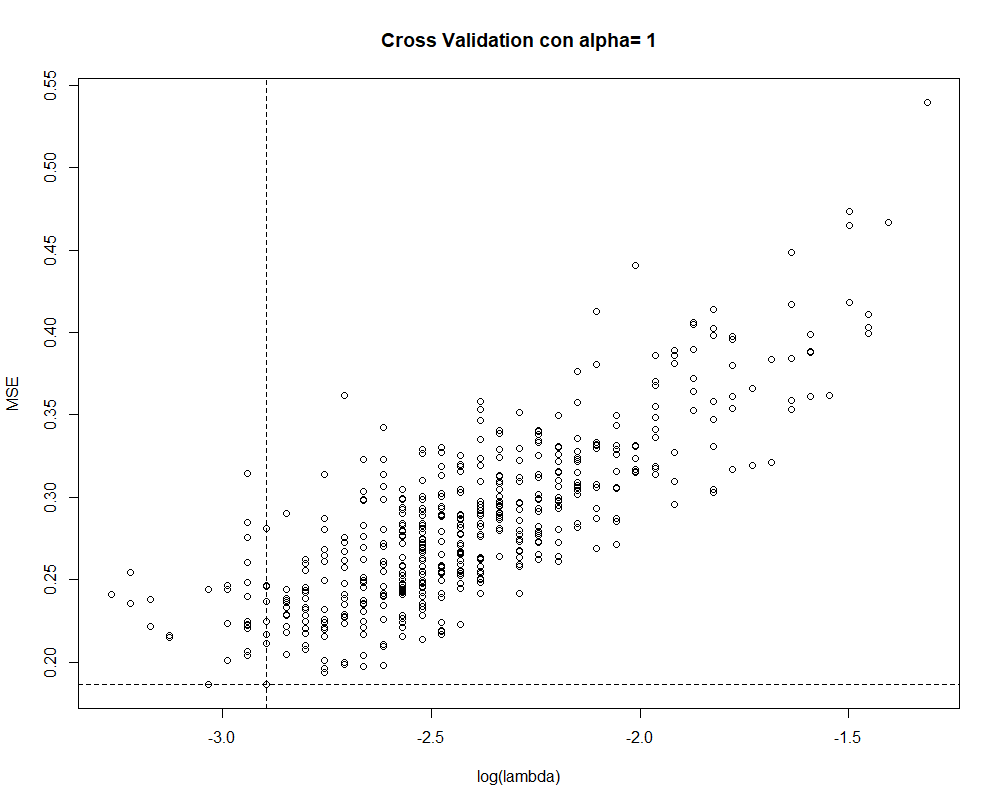
\includegraphics[width=0.48\textwidth]{MSCV3.png}} 
        \caption{}
    \end{figure}
\end{frame}
\begin{frame}{Problema 2: Modelos regularizados}
    \begin{table}[htbp]
        \begin{center}
        \resizebox{\textwidth}{!}{
            \begin{tabular}{c|c|c|c|c|c|c|c|c|c}
                \toprule
                Modelo     &   $mse_{min}$ &  $mse_{1se}$ & $mse_{RCV}$ & $\lambda_{min}$ & $\lambda_{1se}$ & $\lambda_{RCV}$ & $df_{min}$ & $df_{1se}$ & $df_{RCV}$ \\
                \midrule
                Ridge      & 0.26 & 0.29 & 0.24 & 5.93 & 21.82 & 18.98 & 4089 & 4089 & 4089 \\ 
                Elastic Net & 0.24 & 0.30 & 0.19 & 0.10 & 0.24 & 0.13 &  49  & 34 & 45 \\
                Lasso      & 0.18 & 0.22 & 0.18 & 0.039 & 0.08 & 0.05 &  40  & 29 & 34 \\ 
                \bottomrule
                \end{tabular}

        }
        \caption{Errores por validación cruzada}
        \label{tabla:MS}
        \end{center}
    \end{table}
\end{frame}
\begin{frame}{Problema 2: Errores de cada modelo}
    \begin{table}[htbp]
        \begin{center}
        \begin{tabular}{c|p{1.5cm}|p{1.5cm}|p{1.5cm}}
        \toprule
        Modelo       &  Error aparente  &  Error no aparente  & Error no aparente std  \\ 
        \midrule
        Ridge        &     0.079      &      0.29       &  0.027  \\
        Elastic Net   &     0.056      &      0.25       &  0.034  \\
        Lasso        &     0.056      &      0.24       &  0.028  \\
        Modelo nulo  &     0.83       &      0.86       &  0.018  \\
        \bottomrule
        \end{tabular}
        \caption{}
        \label{tabla:ME}
        \end{center}
    \end{table}
\end{frame}
\end{document}